\chapter{基于分布的频率分析攻击方法}
\label{sec:DistributionAttack}

基于分布的攻击利用$\mathbf{C}$和$\mathbf{A}$的数据块的逻辑顺序信息来增强频率分析的有效性。它通过比较$\mathbf{C}$和$\mathbf{A}$的相对频率分布,以减少误报结果。本文还展示了如何利用数据块的大小信息来进一步提高推断精度。

\section{背景知识:基于数据块局部性的频率分析的攻击}

\label{sec:DistributionAttack-prior-attack}

基于分布的频率分析攻击建立在已有的基于数据块局部性的频率分析攻击\citing{li2017information}的基础上,它展示了频率分析如何导致备份工作负载中的信息发生泄漏。基于数据块局部性的频率分析攻击针对每日或每周为主要数据的完整副本(例如,应用程序状态,文件系统快照和VM磁盘映像)创建的完全备份(简称为备份)。它旨在推断不同版本备份间的密文数据块-明文数据块对。它通过假定辅助信息$\mathbf{A}$来自一些较旧的备份,来推断最新备份的明文数据块(即$\mathbf{M}$)。

基于数据块局部性的频率分析攻击利用了数据块局部性这一属性\citing{xia2011silo,zhu2008avoiding,lillibridge2009sparse},这是实际备份工作负载中的常见现象。 具体而言,局部性是指在重复数据删除之前,相邻的数据块在不同版本的备份中往往以相同的逻辑顺序存在。 主要原因是每个备份的更新通常聚集在一些小范围内的数据块中,而剩余的大范围内的数据块在不同版本的备份中保持不变(保持相同的顺序)。

根据局部性原理,基于数据块局部性的频率分析攻击利用逻辑顺序信息来发现密文数据块和明文数据块的邻近信息。具体来说,对于给定的唯一密文数据块$C$,对手首先标识所有相同副本的集合$\{\hat{C}^{(i)}\}$。对于每个$\hat{C}^{(i)}$,它会考虑$\hat{C}^{(i)}$的左右邻居,即$\hat{C}^{(i-1)}$和$\hat{C}^{(i+1)}$。它将左右邻居的集合分别提取到关联数组$\mathbf{L_C}$和$\mathbf{R_C}$中。关联数组分别存储每个唯一密文$C$的映射及其与左右邻居的共现频率。同时,对手还会根据$\mathbf{A}$的逻辑顺序信息构造关联数组$\mathbf{L_A}$和$\mathbf{R_A}$。

然后,基于数据块局部性的频率分析攻击通过每个推断的密文数据块-明文数据块对的邻居进行迭代频率分析。它首先在$\mathbf{C}$(将要进行推测的密文数据块集合)和$\mathbf{A}$(辅助信息-明文数据块的集合)中通过频率分析推断得到出现频率最高的$u$组密文数据块-明文数据块对\{$(C,M)$\}($u$是该攻击开始时用于选取明密文数据块对数量的参数,一般设为5)。因为基于观察得到高频率数据块的频率等级(相对排名)在不同版本的备份中是稳定的,所以推断结果可能是真实的(即,目标密文数据块与推断的明文数据块是正确的唯一映射)。对于每个推断的明密文数据块对$(C,M)$,攻击发现它们的左右邻居$C$和$M$的共现频率最高,由于局部性的原因,$M$的左右邻居可能分别是$C$的相应左右邻居的原始明文数据块。因此,将$C$和$M$的最高频率左(右)邻居添加到推断的密文数据块-明文数据块对的集合中(从存储密文数据块$C$的左右邻居的集合的关联数组$\mathbf{L_C}$和$\mathbf{R_C}$中获得;对于辅助信息:明文数据块$A$,同理,从$\mathbf{L_A}$和$\mathbf{R_A}$中获得)。最后,不断迭代此过程,直到检查完每个推断得到的的密文数据块-明文数据块对的邻居。

因为数据块的顺序由数据块局部性保留,所以它可以使用频率分析来推断在相应的邻居中具有相同的共现频率等级的新的密文数据块-明文数据块对。$M$的左右邻居可能是$C$的相应邻居的原始明文。因此,攻击通过这些新推断的密文数据块-明文数据块对的邻居进一步迭代相同的频率分析,从而增加攻击的严重性。


%\begin{algorithm}
%\caption{Locality-based Attack}
%\label{alg:Locality-basedAttack}
%\small
%   \SetKwFunction{Main}{\sc LOCALITY-BASED ATTACK}
%   \SetKwProg{Pro}{procedure}{:}{}
% 	\Pro{\Main{$C,M,u,v,w$}}{
% 	
% 	$(F_C, L_C, R_C) \longleftarrow COUNT(C)$\;
% 	$(F_M, L_M, R_M) \longleftarrow COUNT(M)$\;
%
%	\If{ciphertext-only mode}{
% 		$\\mathcal{G} \longleftarrow FREQ-ANALYSIS(F_C, F_M, u)$\;
% 	}
% 	\ElseIf{known-plaintext mode}{
% 		$\mathcal{G} \longleftarrow set of leaked ciphertext-plaintext chunk pairs$\;
% 	}
% 	$\mathcal{T} \longleftarrow \mathcal{G}$\;
% 	\While{$\mathcal{G}$ is non-empty}{
%        Remove $(C,M)$ from $\mathcal{G}$\;
% 	  
%        $\mathcal{T}_l \longleftarrow FREQ-ANALYSIS(L_C[C],L_M[M],v)$\; 
%    }
%
%
%\end{algorithm}

然而,基于数据块局部性的频率分析攻击存在一个主要问题:它引入了大量误报(即,不正确的密文数据块-明文数据块对)。 由于频率分析的主要思想是将密文映射到具有相同频率等级的明文,因此对频率等级的任何干扰(例如,跨备份的更新)都可能导致推断出不正确的密文数据块-明文数据块对,这又将导致对其邻居的推断发生错误。虽然基于数据块局部性的频率分析攻击被证明可以有效地推断出真正的密文数据块-明文数据块对的很大一部分,但是对手对于判断每个推断的密文数据块-明文数据块对的真实性置信度较低。例如,根据评估显示,攻击可以在某些情况下可以正确地推断出15.2%的密文数据块-明文数据块对,但在其推断结果中大约65.2%的推断结果是错误的。 


基于数据块局部性的频率分析攻击方法对频率排名非常敏感,如果频率排序受到任何干扰都会极大的降低推断精度。而这些推断错误的明密文数据块对将会干扰到对其相邻数据块的推断迭代过程,导致错误更加严重。即使通过下调参数$u$的大小来限制返回数据块的数量,以提高推断的正确率(仅将频率显著高于其他数据块对的数据块对返回),但会导致推利率的严重下滑(推断得到的数据块对总数大幅减少)。

\section{基于分布的频率分析攻击方法定义}
\label{sec:distribution-attack-description}

基于分布的频率分析攻击的攻击扩展了基于数据块局部性的频率分析攻击\cite{li2017information}以显著消除误报。它利用备份工作负载中的数据块局部性性,就像基于数据块局部性的攻击一样。在基于数据块局部性的攻击的基础上,对于$\mathbf{C}$中的每个唯一密文$C$,根据该数据块与其邻居的共现频率来测量其相对频率分布;同时,用同样的方法计算$\mathbf{A}$中每个唯一明文$M$的相对频率分布。根据观察,对于推断正确的密文数据块-明文数据块对$(C,M)$,$C$和$M$应该具有相似的相对频率分布(即,它们与它们各自的邻居的共现频率是相似的)。对于此的理解是,如果$M$是$C$的原始明文,那么$M$和$C$的相对频率分布可能是相似的。 基本原理是$\mathbf{A}$和$\mathbf{C}$从同一个源映射得到,因此具有大量未被修改的数据块,所以相对频率分布得到保留。本文将此观察视为局部性属性的更一般化概念,并根据该条件过滤可能不正确的密文数据块-明文数据块对,以提高推断的准确性。

\begin{figure}[!htb]
    \small
    \centering
    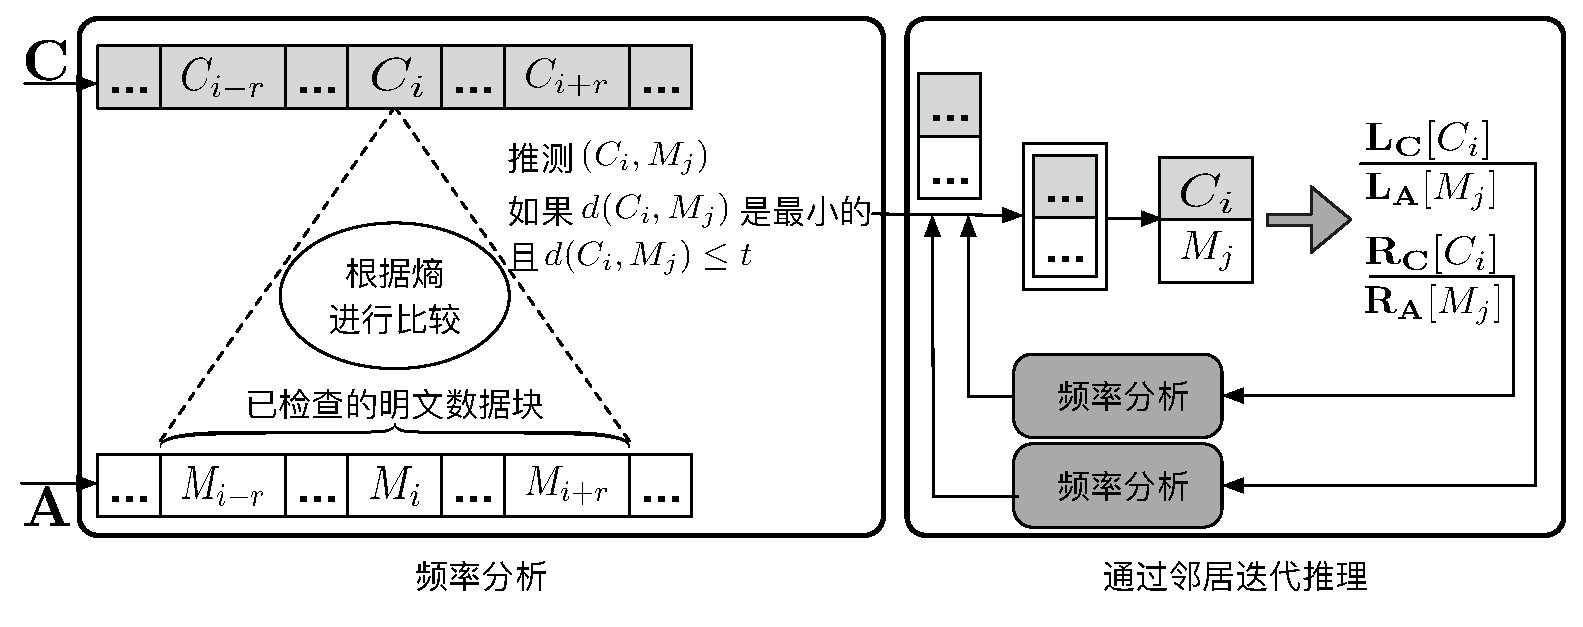
\includegraphics[width=14cm]{DistributionAttack}
    \caption{基于分布的频率分析攻击工作流程} 
    \label{fig:基于分布的频率分析攻击工作流程}
\end{figure}

图\ref{fig:基于分布的频率分析攻击工作流程}展示了基于分布的频率分析攻击方案的工作流程。

首先按$\mathbf{C}$和$\mathbf{A}$中的频率对具有唯一性的密文和明文进行排序。 与基于数据块局部性的频率分析攻击\citing{li2017information}一样,通过参数$u$将基础频率分析配置为最多返回$u$个频率最高的明密文数据块对。

接下来,对于每个具有唯一性的密文数据块$C_i$(其中$i, 1 \leq i \leq u$,代表了该密文数据块的频率排名),检查相近频率排名范围内明文数据块$M_{i-r}, \ldots, M_i, \ldots, M_{i+r}$(从$i-r$到$i+r$),其中$r$是可配置参数(默认为10),表示可以解决的频率排名干扰的最大范围。

对于每个$C_i$(其中$1 \leq i \leq u$)和相应的$M_j$(其中$i-r\le j\le i+r$),我们通过熵来表示它们的相对频率分布,熵是信息理论中的一个关键概念,用于衡量随机来源产生的信息量。在这里,我们采用熵来量化概率分布的随机性\citing{wang08}。 具体来说,我们定义了两个随机变量,分别用$X$和$Y$来描述$C_i$与其左右邻居的共现事件,这样事件“$X = C$” 表示$C$是$C_i$的左邻居,而事件$Y = C$表示$C$是$C_i$的右邻居。 因此,我们基于$\mathbf{L_C}$和$\mathbf{R_C}$来计算两个事件发生的概率:

\begin{eqnarray}
    \Pr[X = C] = \frac{\mathbf{L_C}[C_i][C]}{\sum_{C' \in \mathbf{L_C}[C_i]} \mathbf{L_C}[C_i][C']}, \nonumber \\
    \Pr[Y = C] = \frac{\mathbf{R_C}[C_i][C]}{\sum_{C' \in \mathbf{R_C}[C_i]} \mathbf{R_C}[C_i][C']}, \nonumber
\end{eqnarray}

其中$\mathbf{L_C}[C_i]$和$\mathbf{R_C}[C_i]$分别了存储$C_i$的左右邻居,而$\mathbf{L_C}[C_i][C']$和$\mathbf{R_C}[C_i][C']$存储$C_i$与其左右邻居$C'$的共现频率。$X$和$Y$都遵循$C_i$的相对频率分布,本文用$e(\mathbf{L_C}[C_i])$和$e(\mathbf{R_C}[C_i])$表征它们的随机性,分别为:

\begin{eqnarray*}
    e(\mathbf{L_C}[C_i]) = \sum_{C \in \mathbf{L_C}[C_i]} \log_2\frac{1}{\Pr[X = C]}, \\
    e(\mathbf{R_C}[C_i]) = \sum_{C \in \mathbf{R_C}[C_i]} \log_2\frac{1}{\Pr[Y = C]}. 
\end{eqnarray*}

类似的,本文根据$\mathbf{L_A}$和$\mathbf{R_A}$对每个明文数据块$M_j$(其中$i-r\le j\le i+r$)计算出其对应的熵$e(\mathbf{L_A}[M_j])$和$e(\mathbf{R_A}[M_j])$,然后本文利用欧几里得距离来量化$C_i$和$M_j$的相对频率分布的相似性,记为$d(C_i, M_j)$:

\begin{equation}
    \label{eq:dis-dcm}
    \centering
    d(C_i, M_j) = \sqrt{[e(\mathbf{L_C}[C_i]) - e(\mathbf{L_A}[M_j])]^2 + [e(\mathbf{R_C}[C_i]) - e(\mathbf{R_A}[M_j])]^2}.
\end{equation}

显然,只有当他们的熵的欧几里德距离$d(C_i, M_j)$很小时,$C_i$和$M_j$才有相似的相对频率分布。因此,如果满足以下条件,则可将$(C_i, M_j)$标识为推断成功的密文数据块-明文数据块对:

\begin{itemize}
\item \textbf{R1:} $d(C_i, M_j)$ 在$j \in i-r \leq j \leq i+r$ 中取到最小值。
\item \textbf{R2:} $d(C_i, M_j)$ 不大于预先设定的变量$t$(例如,$t$的默认值为1)。
\end{itemize}

值得注意的是,$C_i$所对应的原始明文数据块可能不在检查的明文数据块$M_{i-r}, \ldots, M_{i+r}$的范围内。在这种情况下,部分$M_j$($i-r \leq j \leq i+r$)可能仍然满足条件R1。这种情况下,本文希望通过R2过滤不正确的密文数据块-明文数据块对。 

然后,继续采用先前基于数据块局部性的频率分析攻击\citing{li2017information}中的迭代方法(参见章节:\ref{sec:DistributionAttack-prior-attack})来扩展推断的密文数据块-明文数据块对的覆盖范围。具体来说,对于每个推断的$(C_i, M_j)$,应用基于分布的频率分析方案(见上文)通过$C_i$和$M_j$的邻居迭代推断出更多的密文数据块-明文数据块对,在没有新的密文数据块-明文数据块对可以被推断时停止迭代,最终完成基于分布的频率分析攻击的全部过程。
 
\subsection{基于分布的频率分析攻击方法总结} 

总而言之,基于分布的频率分析攻击通过在频率分析中考虑相对频率分布来提供更一般化的局部性概念。它通过三个参数进行配置和调整:

\begin{itemize}
    \item $u$:确定通过频率分析返回的密文数据块-明文数据块对的最大数量。
    \item $r$:确定要考虑的扰动范围的最大值。
    \item $t$:确定欧几里德距离的阈值以过滤可能不正确的推断结果。 
\end{itemize}


先前基于数据块局部性的频率分析攻击\citing{li2017information}可以被视为基于分布的频率分析攻击在$r=0$的参数配置下(即没有处理频率排名中的任何干扰)和$t \rightarrow \infty$(即没有过滤任何不正确的推理结果)的特殊情况。

\section{对数据块大小信息泄漏的利用}

本文提出了基于分布的频率分析攻击的高级变体,它使用数据块大小信息来进一步减少误报。具体来说,假设$\mathbf{C}$中每个密文数据块的大小反映了其原始明文数据块的大小。 

本文的想法建立在这样一个基本事实的基础上:如果密文$C$对应于明文$M$,则$C$的大小近似于$M$的大小。 这是因为加密重复数据删除在要加密的内容中保留了块(即,由对称加密操作的基本单元)的数量信息。 本文通过使用这个事实来进一步过滤不正确的密文数据块-明文数据块对$(C,M)$($C$和$M$中的块数不同)。

在本课题中,假设每个块的大小都是16字节(AES加密的典型配置)。对于每个经过基于分布的频率分析攻击方法得到的明文数据块-密文数据块对$(C_i, M_j)$,分别将$C_i$和$M_j$中的块数导出为$b({C_i})$和$b({M_j})$:

\begin{eqnarray*}
b({C_i}) = \lceil \frac{{\sf size}(C_i)}{16} \rceil, \nonumber \\
b({M_j}) = \lceil \frac{{\sf size}(M_j)}{16} \rceil, \nonumber 
\end{eqnarray*}

其中${\sf size}(C_i)$和${\sf size}(M_j)$分别是$C_i$和$M_j$的确切大小, $\lceil x \rceil$ 返回了大于或等于$x$的最小整数。在基于分布的频率分析攻击中提出的过滤条件R1和R2(参见章节:\ref{sec:distribution-attack-description})的基础上,给出以下过基于数据块中块数信息的滤条件:  
 
\begin{itemize}[leftmargin=*]
    \item {\bf R3:} $b({C_i})$ equals $b({M_j})$.
\end{itemize}

对于使用可变大小的数据分块方法的加密重复数据删除中,不同的数据块可能具有不同的大小,因此使用R3可以有效进行过滤。然而,在使用固定大小的数据分块方法的机密重复数据删除中,R3对于任意一组$(C, M)$始终成立。但此时,仍然可以通过应用R1和R2来提高频率分析攻击的精度。
     

\section{本章小结}

本章介绍了本文提出的第一种改进的频率分析方法:基于分布的频率分析攻击方法。给出了该方法的形式定义、方法描述以及对数据块大小信息泄漏的扩展利用方法。                  



